\appendixpage
\addappheadtotoc

\pagestyle{plain}
\chapter{Authenticators}

This chapter describes setting up an authenticator app for Two Factor Authentication (2FA) to be used with Obidos.
2FA makes it harder for someone to maliciously change a user's passphrase or local password.
Since changing the passphrase can destroy existing entities created by the User, it is very important to make sure
the authenticity of the User in such a point-of-no-return situation. 2FA essentially gives an extra level of verification.
\newline
\tab Either Google Authenticator or Authy can be used with Obidos. 
Both these apps are available from Google Play for Androids and from iTunes for iPhones.
Google Authenticator is very simple and easy to use. Once set up, it can work even when there is no Internet connection.
Authy is a bit more sophisticated. To configure Authy you need a cell\# and an email address.
If you lose your phone, you can set up Authy on the desktop using the same cell\# and email. That way the configuration
set up for Obidos can be salvaged in case the phone is lost. This is because Authy allows backing up to cloud.
In the following sections we give an outline of setting up both these apps.

\section{Google Authenticator}
Once logged into iTunes, if a search for 'Google Authenticator' will show a screen similar to the following.
The app can be download by clicking on the 'OPEN' button. 

\begin{figure}[H]
\centering
\fbox{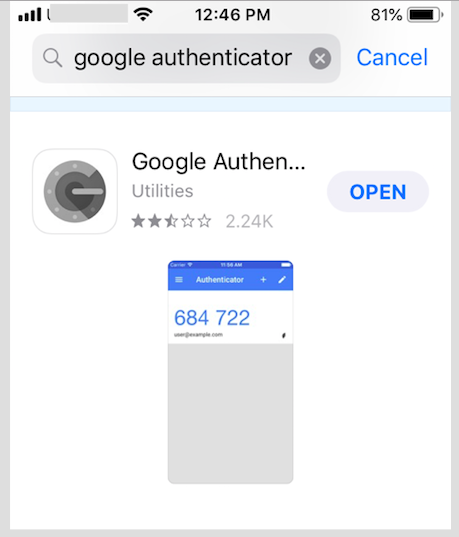
\includegraphics[scale=0.35]{user/Google-Auth-iTunes.png}}
\caption{Google Authenticator in iTunes}
\label{fig: Figure}
\end{figure}

After installing, when opening Google Authenticator, the very first screen will look similar to the 
following figure. Click on 'BEGIN SETUP'.

\begin{figure}[H]
\centering
\fbox{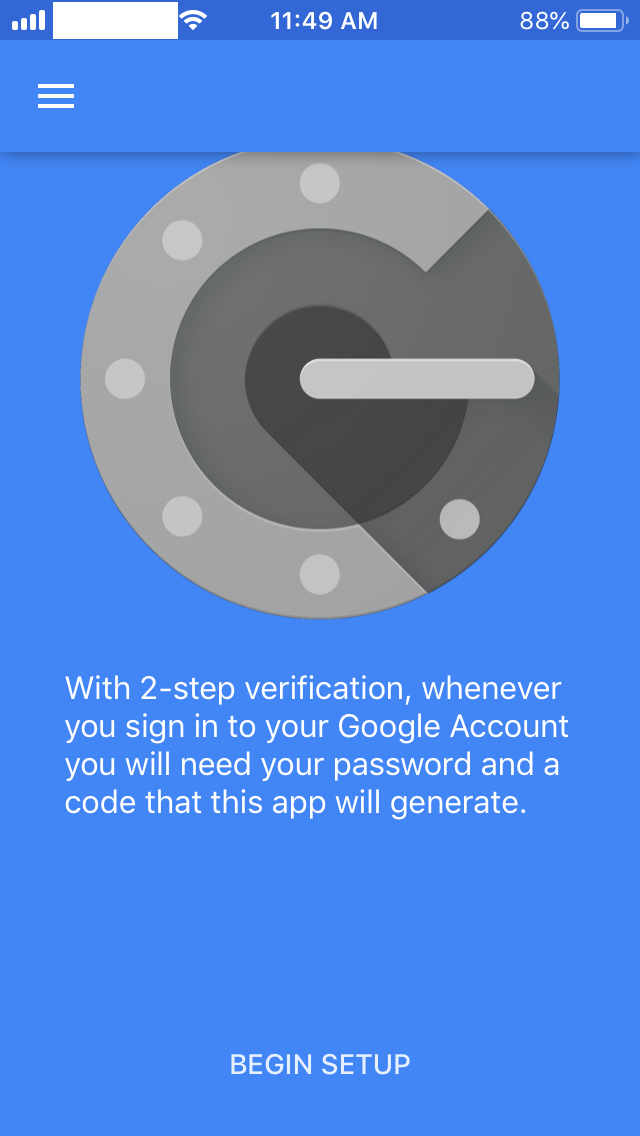
\includegraphics[scale=0.2]{user/Goog-Auth-1.png}}
\caption{Google Authenticator Initial screen}
\label{fig: Figure}
\end{figure}

During setup, there are two options. One is to scan a QR code and the other is to manually
enter the code from Obidos.

\begin{figure}[H]
\centering
\fbox{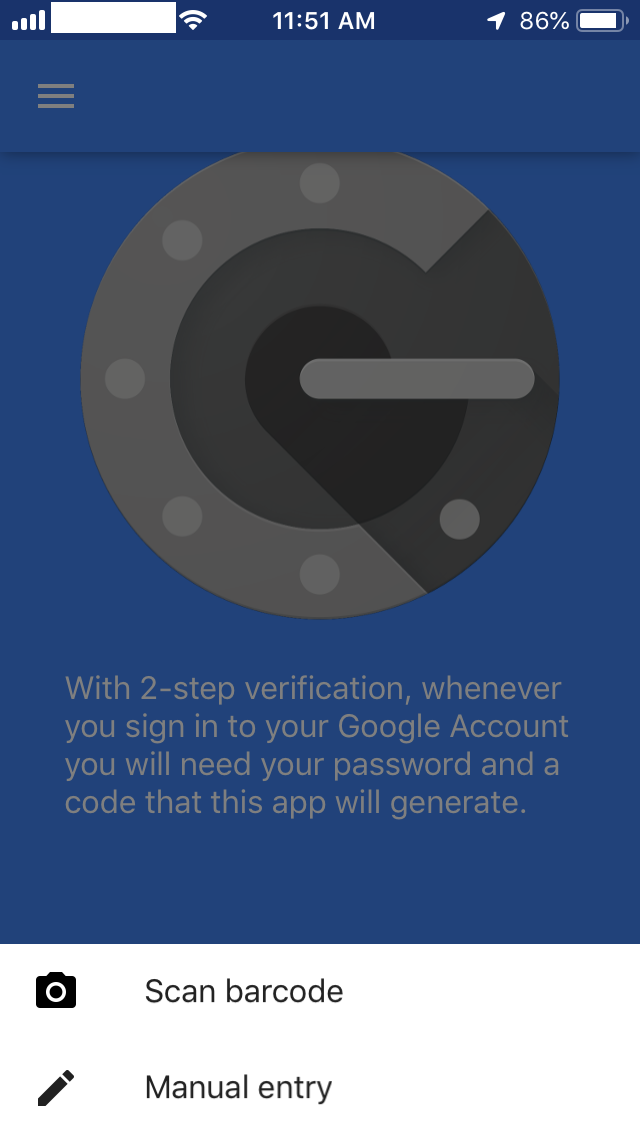
\includegraphics[scale=0.2]{user/Goog-Auth-2.png}}
\caption{Screen to choose between Scanning QR code or entering code manually}
\label{fig: Figure}
\end{figure}

Obidos displays both QR code and the text code. So either the QR code from Obidos can be scanned or
the text code can be manually entered. When the option to scan QR code is selected, the camera will come into focus.
The phone position must be adjusted so that the QR code comes within the green square.

\begin{figure}[H]
\centering
\fbox{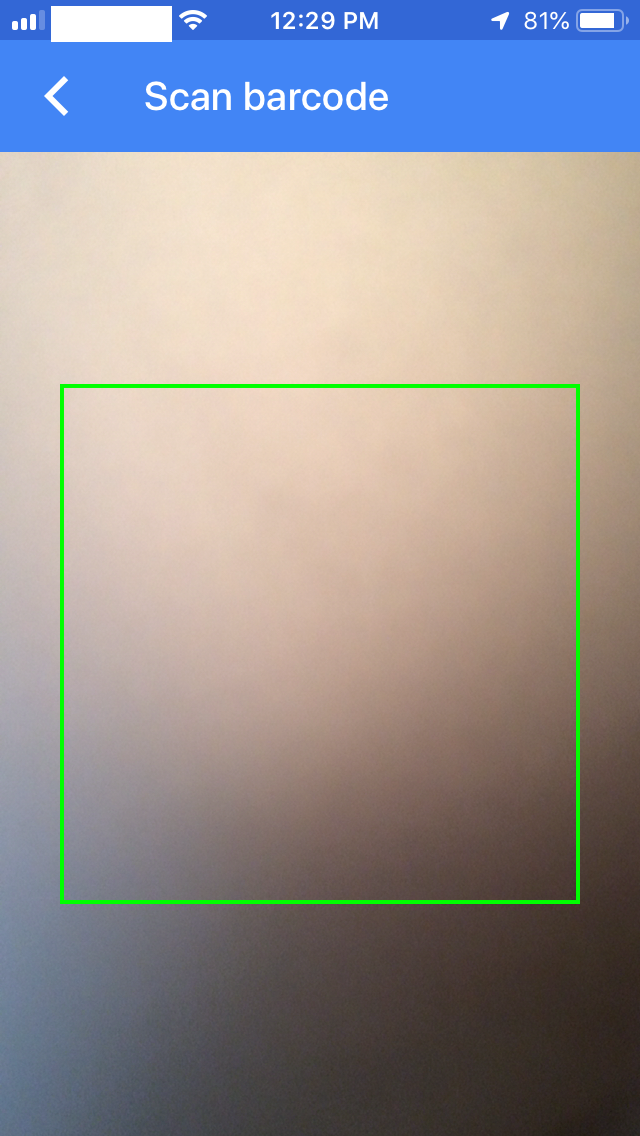
\includegraphics[scale=0.2]{user/Goog-Auth-3.png}}
\caption{QR Code Scanning Frame}
\label{fig: Figure}
\end{figure}

After scanning the QR code from Obidos (or manually entering the code), the Authenticator screen 
will look as in the following figure. 
A six digit code will be displayed and this code will change every 30 seconds.
This is the code that is requited by Obidos whenever 2FA authentication is used.

\begin{figure}[H]
\centering
\fbox{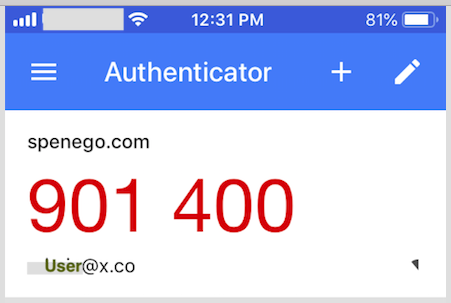
\includegraphics[scale=0.4]{user/Goog-Auth-4.png}}
\caption{Google Authenticator 6 digit code}
\label{fig: Figure}
\end{figure}

\pagebreak

\section{Authy}
In iTunes, searching for 'Authy' will show a screen similar to the following.
Download Authy by clicking on the 'OPEN' button. 

\begin{figure}[H]
\centering
\fbox{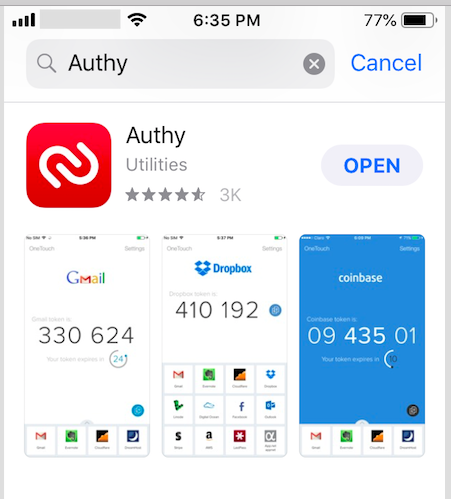
\includegraphics[scale=0.3]{user/Authy-iTunes.png}}
\caption{Authy in iTunes}
\label{fig: Figure}
\end{figure}

When 'Authy' is initially opened, the setup screen will start configuration by asking for cell phone number.
Once the phone number is entered, an email address will need to be provided.

\begin{figure}[H]
\centering
\fbox{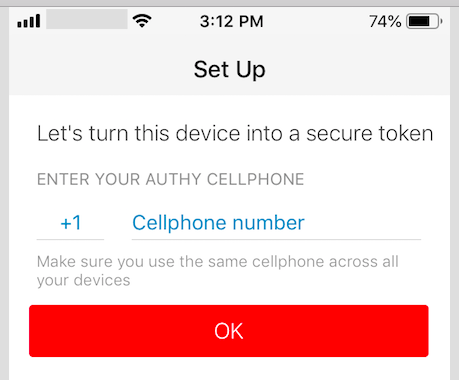
\includegraphics[scale=0.3]{user/Authy-1.png}}
\caption{Authy setup screen}
\label{fig: Figure}
\end{figure}

After entering initial information, Authy will provide you a confirmation code via phone call
or via SMS text. User will be given the choice.

\begin{figure}[H]
\centering
\fbox{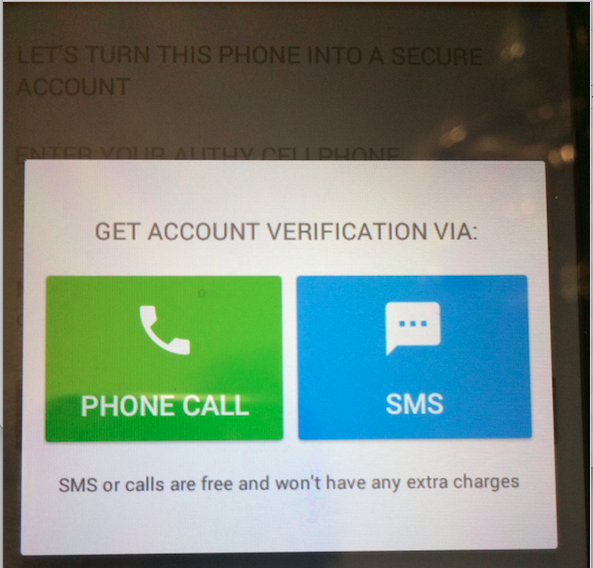
\includegraphics[scale=0.35]{user/Authy-2.png}}
\caption{Mode of communicating confirmation code}
\label{fig: Figure}
\end{figure}

After dispatching the code, Authy will ask the User to enter the confirmation code.

\begin{figure}[H]
\centering
\fbox{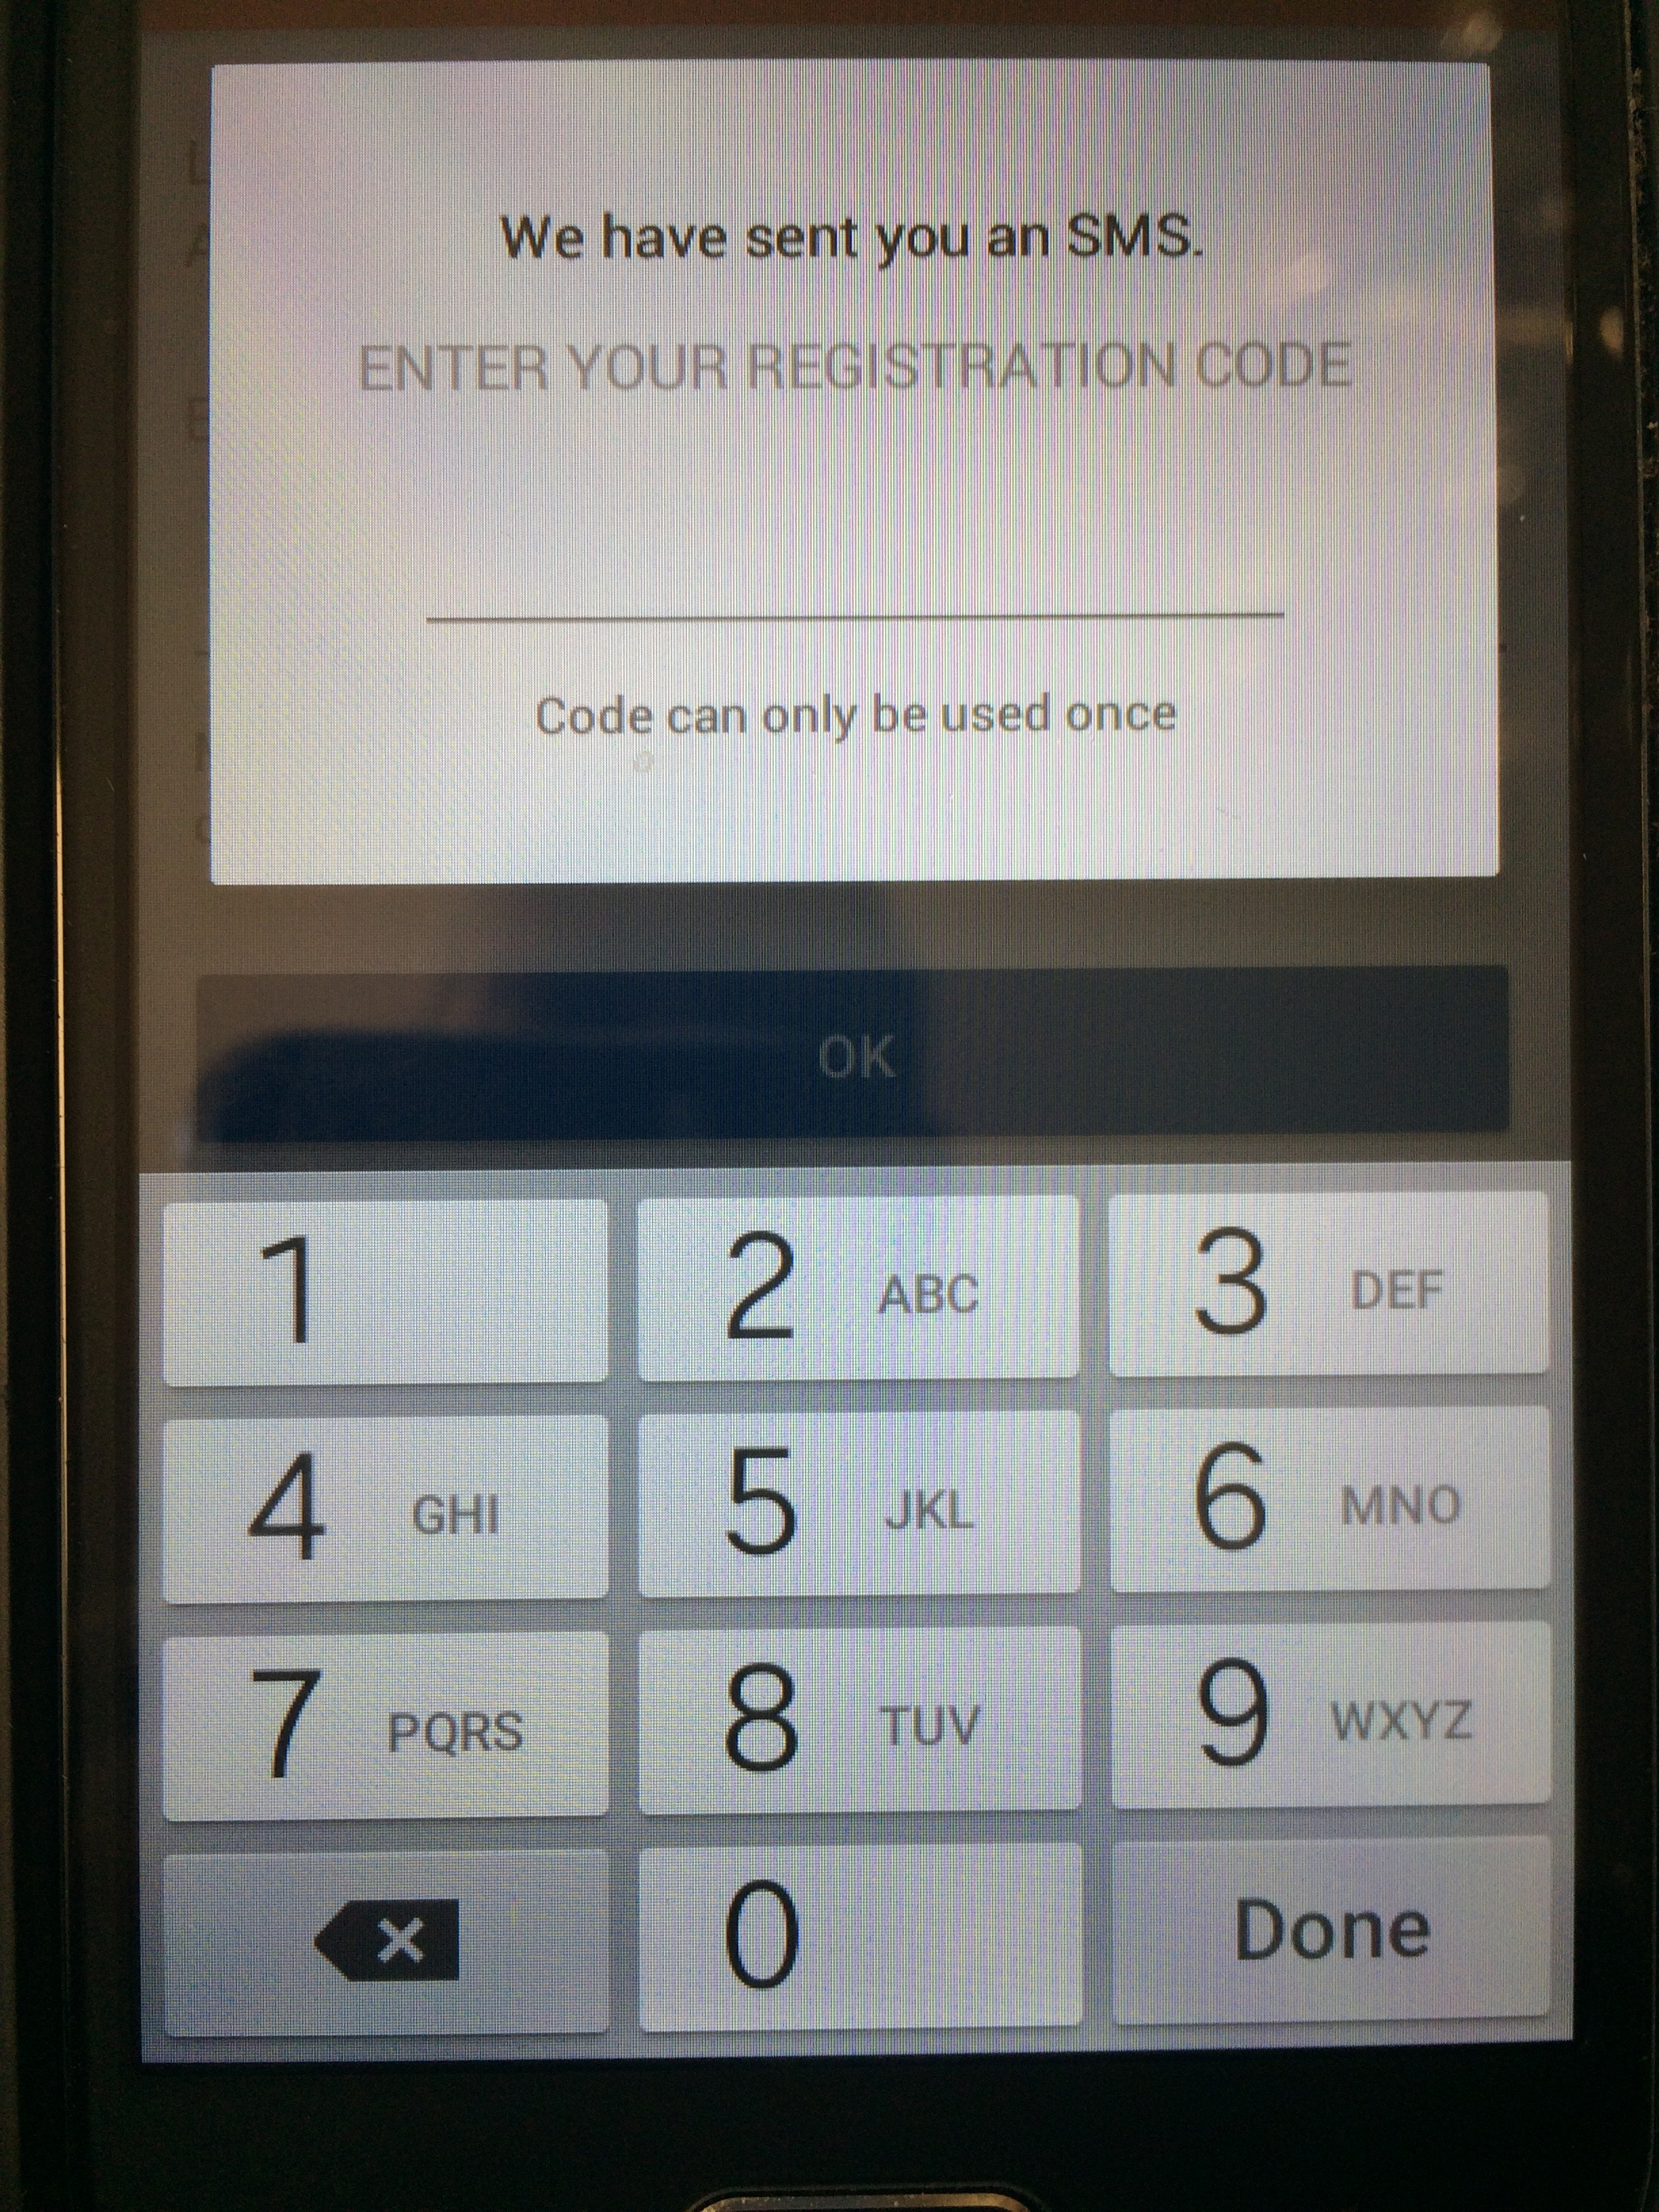
\includegraphics[scale=0.08]{user/Authy-3.jpg}}
\caption{Screen for entering the confirmation code}
\label{fig: Figure}
\end{figure}

Once the confirmation code is validated, it is ready to set up authenticator accounts.

\begin{figure}[H]
\centering
\fbox{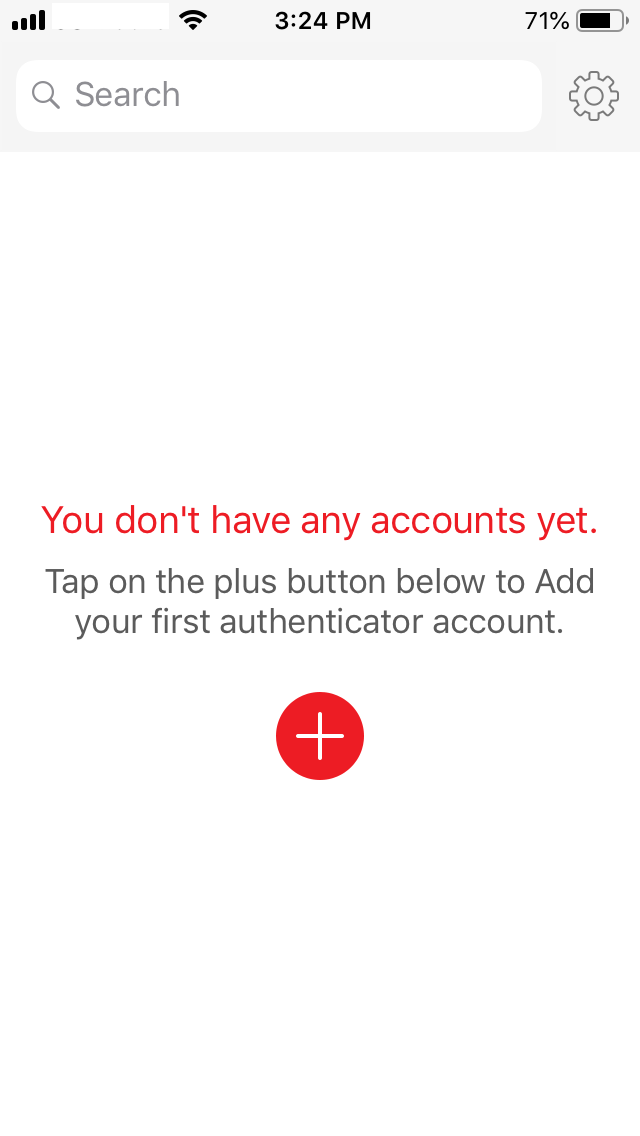
\includegraphics[scale=0.2]{user/Authy-4.png}}
\caption{Ready to set up authenticator accounts}
\label{fig: Figure}
\end{figure}

Press the + button to get started. Now the option to scan a QR code or manually enter a code is seen.

\begin{figure}[H]
\centering
\fbox{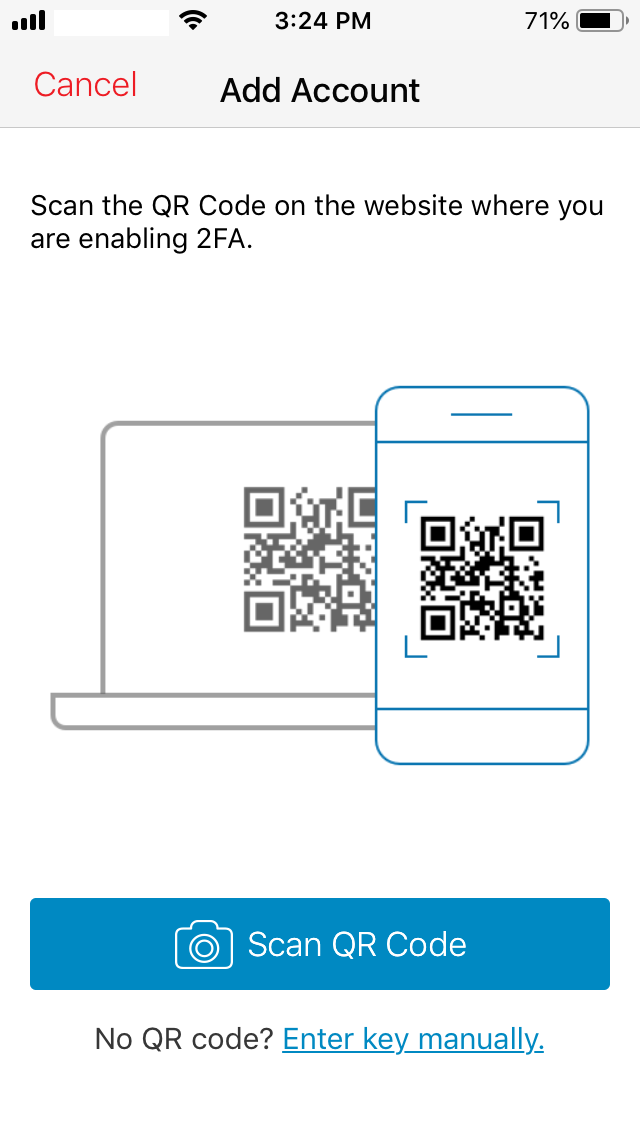
\includegraphics[scale=0.22]{user/Authy-5.png}}
\caption{Enter code from Obidos}
\label{fig: Figure}
\end{figure}

When the code is entered (or scanned in), Authy gives you the option to save your configurations in the cloud.

\begin{figure}[H]
\centering
\fbox{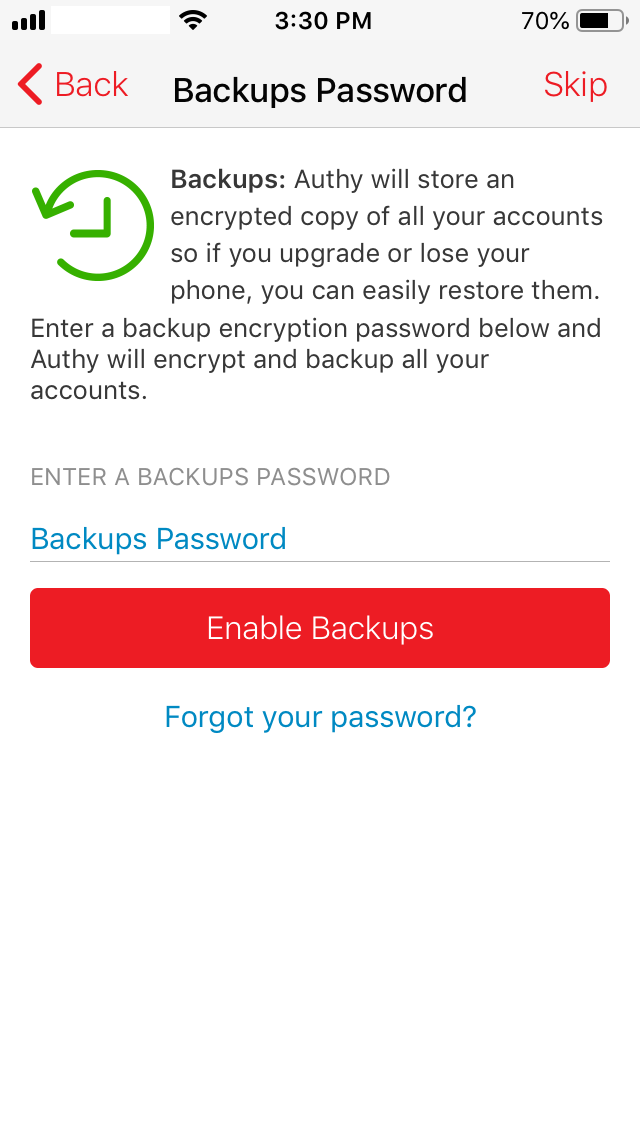
\includegraphics[scale=0.22]{user/Authy-6.png}}
\caption{Cloud backup option}
\label{fig: Figure}
\end{figure}

And finally the scanned code information is presented.

\begin{figure}[H]
\centering
\fbox{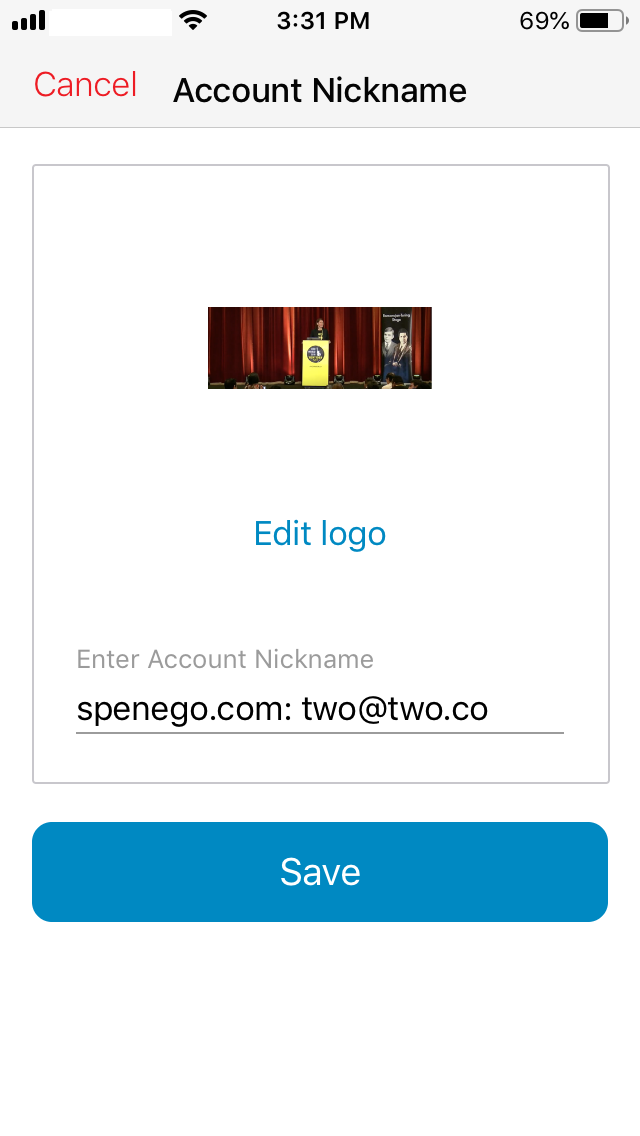
\includegraphics[scale=0.2]{user/Authy-7.png}}
\caption{Save the settings}
\label{fig: Figure}
\end{figure}

Once you save the information, the 6 digt code is displayed. This is the code that Obidos requires when 2FA is used.

\begin{figure}[H]
\centering
\fbox{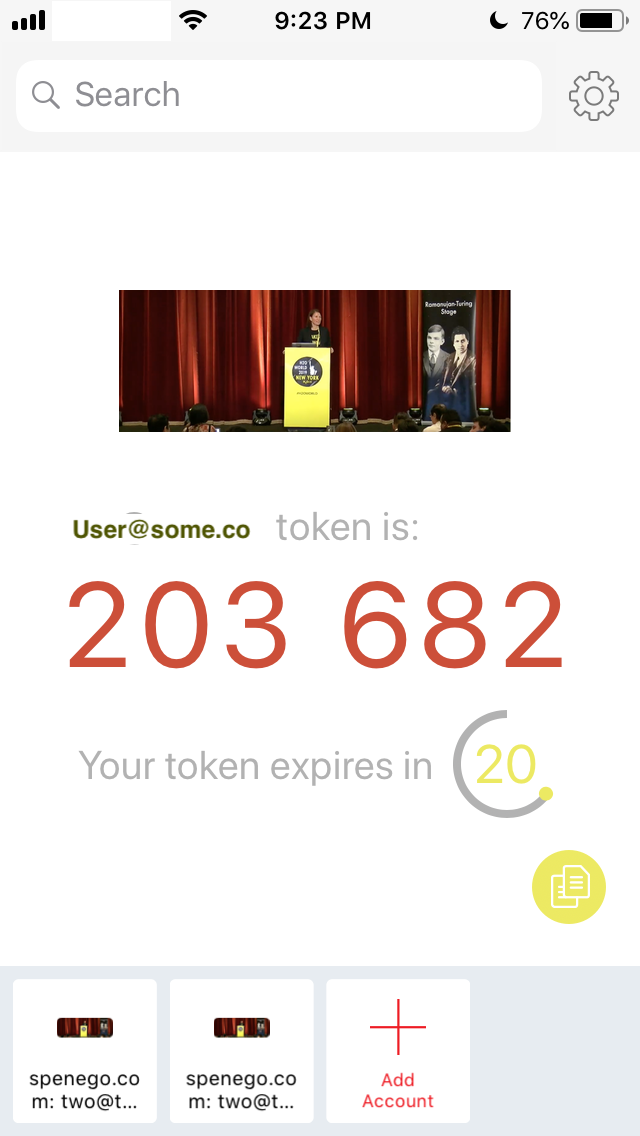
\includegraphics[scale=0.2]{user/Authy-8.png}}
\caption{Authy 6 digit code display}
\label{fig: Figure}
\end{figure}
